Given equation of the line, 
\begin{align}
\myvec{k-3 & -(4-k^2)}\vec{x}+k^2-7k+6=0\label{oct/2/106/eq:1}\end{align}
of a general line equation \begin{align}{\vec{nx} = c}\end{align}\newline
here \begin{align}{\vec{n} =\myvec{k-3 & -\{4-k^2\}}}\newline\end{align}
and \begin{align}{c = -k^2+7k-6}\end{align}
\begin{enumerate}[label=\emph{\alph*)}]
\item Parallel to x-axis
\begin{align}
\vec{n}=\myvec{0 & 1}\end{align}if the line is parallel to x-axis
Equation of x-axis is \begin{align}\begin{split}\myvec{1 & 0}\vec{x}& =0\\
 \myvec{1 & 0}\myvec{k-3\\-\{4-k^2\}} & = 0 \label{oct/2/106/eq1}\\
  k-3 & = 0\\
    \implies k & =3
\end{split}\end{align}
Substituting $k=3$ in \eqref{oct/2/106/eq:1}
Equation of line is,
\begin{align}
     \myvec{0 & 5}\vec{x}=6
\end{align}
 
\item Parallel to y-axis
 \begin{align}\vec{n} & =\myvec{1 & 0} \end{align} if the line is parallel to y-axis Equation of y-axis is  \begin{align}\begin{split}\myvec{0 & 1}\vec{x} & =0\\
\myvec{0 & 1}\myvec{k-3\\-(4-k^2)} & = 0\\ \label{oct/2/106/eq1}
 4-k^2 & =0\\
 \implies k & =\pm2
\end{split}
\end{align}
Substituting $k=2$ in \eqref{oct/2/106/eq:1}.
Equation of line is,
\begin{align}
     \myvec{-1 & 0}\vec{x} & = 4
\end{align}
Substituting $k=-2$ in \eqref{oct/2/106/eq:1}.
Equation of line is,
\begin{align}
  \myvec{-5 & 0}\vec{x} & =-24
\end{align}
\item Passing through origin 
${c = 0}$ if the line passes through origin
Equation of line when passing through origin is 
\begin{align}
\vec{n}^\top\vec{x} & =0
\end{align}
Hence
\begin{align} \label{oct/2/106/eq1}
\begin{split}
-k^2+7k-6 & = 0\\
 & = -k^2+k+6k-6\\
 & =(k-1)(k-6)\\
\implies k&=1, k=6
\end{split}
\end{align}
Substituting $k=1$ in \eqref{oct/2/106/eq:1}.
The equation of line is,
\begin{align}
\myvec{-2&-3}\vec{x} = 0
\end{align}
Substituting $k=6$ in \eqref{oct/2/106/eq:1}.
The equation of line is,
\begin{align}
  \myvec{3 & 32}\vec{x} = 0
\end{align}
\end{enumerate}
\begin{figure}[!h]
         \centering
         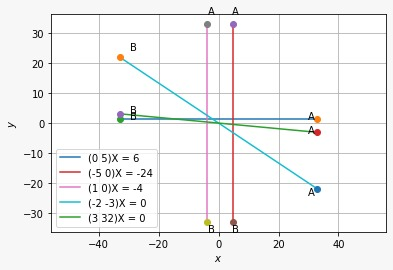
\includegraphics[width=\columnwidth]{solutions/oct/2/106/figure L.jpeg}
         \caption{Plot of line equations}
         \label{oct/2/106/fig:x cubed graph}
\end{figure}
